\documentclass[a4paper,10pt]{article}
\usepackage[utf8]{inputenc}
\usepackage{graphicx}
\usepackage{hyperref}
\usepackage{geometry}
\geometry{
	a4paper,
	left=13mm,
	right=13mm,
	top=13mm,
	bottom=13mm,
}
\usepackage{caption}
\usepackage{subcaption}
\usepackage[toc,page]{appendix}


\title{Fully dynamic k-center clustering\\
 \vspace{0.3cm}
	\small Project report}
\author{Adèle Mortier}

\begin{document}



\maketitle
\section*{Introduction}
The aim of this class project was to implement an algorithm that maintains efficiently and cheaply a clustering for GPS-located tweets that had been collected on Twitter. The algorithm was based on a popular method called $k$-center clustering (or $k$-means clustering). Contrary to a standard $k$-means problem, the data were dynamic in the sense that at each step, the oldest tweet was removed from the dataset and the newest was added. For our implementation, we used Python and the following combinations of parameters :
\begin{center}
	\begin{tabular}{| c | c | c |}
		\hline
		Variable & Name & Value \\ \hline
		Number of clusters & \texttt{k} & $[15, 20]$ \\
		Dataset size & \texttt{window\_width} & $[10 000, 15 000]$ \\
		Number of updates\footnote{one update is composed of one tweet insertion and one tweet deletion} & \texttt{n\_operations} & $60000$\\
		\hline
	\end{tabular}
\end{center}

\section{Project description}
	\subsection{Preprocessing}
		The data had been stored in a \texttt{txt} file, each line of the file representing a tweet (\textit{i.e.} a timestamp, a latitude and a longitude). We parsed this file and put the data in a \texttt{h5} file\footnote{using the package \texttt{h5py}} to have faster I/O for our later queries on the dataset. We also put a unique \textit{id} (basically, an \texttt{int}) on each tweet to manipulate them more abstractly and efficiently. The data (latitude, longitude) behind each tweet \textit{id} could be easily retrieved using a Python dictionary.
	\subsection{Computation of the dataset parameters}
		Before doing the clustering, we had to retrieve two parameters from our dataset, which were :
		\begin{eqnarray*}
			d_{min} = min_{x_1 \neq x_2 \in S}\left(dist(x_1, x_2)\right) \\
			d_{max} = max_{x_1 \neq x_2 \in S}\left(dist(x_1, x_2)\right)
		\end{eqnarray*}
		$S$ being the set of tweets defined by their GPS coordinates. We wanted $dist$ to be a relevant metric w.r.t our data, so we used a custom metric called the Haversine distance that computes the distance (in kilometers) between two points defined by their GPS coordinates.\\
		To compute $d_{min}$ and $d_{max}$, we first tried a brute-force method that consisted in using the Scipy \texttt{pdist} function that computes the pairwise distance for all points i a dataset\footnote{and then we would have taken the minimum and the maximum of these distances}. But the function ran out of memory when computing on the $1$ million tweets.\\
		We thus chose more refined methods, \textit{i.e.} Delaunay triangulation \cite{Delaunay1934} for $d_{min}$ and Rotating calipers \cite{Shamos1978} for $d_{max}$. We took code snippets from \href{https://stackoverflow.com/questions/5119644/identifying-points-with-the-smallest-euclidean-distance}{here} and \href{https://www.ics.uci.edu/~eppstein/161/python/diameter.py}{here} and adapted them such that we could deal with the Haversine distance instead of the Euclidean one. The Delaunay (D) algorithm and the Rotating calipers (RC) algorithm returned the following results :
		\begin{center}
			\begin{tabular}{| c | c | c |}
				\hline
				Algorithm & Expected result & Value (km)\\ \hline
				D & $d_{min}$ & $8.50586308516 \times 10^{-7}$ \\
				RC & $d_{max}$ & $18680.1424983$ \\
				\hline
			\end{tabular}
		\end{center}
		The values compiled above look consistent with our metric and the Earth topology : we expected the upper bound of $d_{max}$ to be about $20000$ km\footnote{half the Earth's circumference}, and the lower bound of $d_{min}$ to be close to zero\footnote{tweets written by the same person...}. With these values is was then easy to compute the different values of $\beta$ for each value of $\epsilon$
	\subsection{Algorithms}
		We implemented the algorithms as specified in \cite{Chan2017}. More precisely :
		\begin{itemize}
			\item for a fixed $\beta$, a ($\beta$-)clustering is a Python \texttt{dict}, whose keys are the tweet \textit{ids}\footnote{for the tweets that belong to the current dataset}, and whose values are the centers \textit{ids}. Each tweet \textit{id} is then mapped to the cluster it belongs to (identified by the \textit{id} of its center), or to $-1$ if it is not yet clustered.
			\item for a set of $\beta$\begin{tiny}s\end{tiny}, a $\beta$\begin{tiny}s\end{tiny}-clustering is a \texttt{dict} that maps each $\beta$ to its corresponding clustering.
			\item for a set of $\epsilon$\begin{tiny}s\end{tiny}, an $\epsilon$-clustering is a \texttt{dict} that maps each value of $\epsilon$ to its corresponding $\beta$\begin{tiny}s\end{tiny}-clustering
		\end{itemize}
		We used the \texttt{dict} structure for two reasons : first the \texttt{dict} structure is more modular\footnote{for instance if we wanted to do something else than the sliding window model, \textit{e.g.} add/remove the nodes in random order (and hence by random \textit{id}), a \texttt{dict} would be much more convenient (w.r.t a \texttt{list}) to remember which point belong to which cluster...}, second because of the good time complexities of this structure\footnote{for \texttt{get} and \texttt{set}, both the \texttt{dict} and the \texttt{list} are $O(1)$ on average. \texttt{dict} is better on average for \texttt{delete}, with a $O(1)$, \textit{vs} $O(n)$ for the \texttt{list}. That is good for us because we have to do as many deletions as insertions in our framework. Conversely, we do not use so many times \texttt{get} and \texttt{set}, where the \texttt{list} is slightly better (in worst case).}
\section{Analysis}
All the plots and tables are in the Appendix.
	\subsection{Time}
		As we look at Figure \ref{maps}, the algorithm seems to work well, and the Haversine metric allows to see a real geographical clustering, with areas that coincide with the different continents and the regions within them that present a huge demographic density : US East- and Westcoasts, Europe, East-Asia, Middle-East, South-Africa, South America... We can notice that the partition is quite robust regarding reclustering after center deletion. The clusters that keep the same color have not been reclustered, whereas there is a brand new cluster located in Japan, and for instance the Australian cluster has moved a bit.\\
		As we look at the plots of Figure \ref{plots}, we can observe that the execution time is very sensitive to the precision parameter $\epsilon$. Indeed, a smaller $\epsilon$ (\textit{i.e.} a higher precision) forces us to compute a clustering for more $\beta$\begin{tiny}s\end{tiny}, and thus the computation takes more time... The time is also sensitive to the number of clusters : adding $5$ clusters increases the computation time by $13\%$ on average for each $\epsilon$.
	\subsection{Accuracy}
		We did two measures for accuracy. Both relied on the following assumptions :
		\begin{itemize}
			\item a static clustering (without any insertions/deletions) on a given window is a ground truth for this window;
			\item an approximation for a ``target'' window is obtained by ``sliding'' another window located at the beginning of the dataset to this target window using insertion/deletions.
		\end{itemize}
		We computed the F1 score\footnote{as defined in the course on Community detection, slides 24-25} of different approximations w.r.t a clustering on the target window $[50k; 60k[$, with a number of $15$ clusters. An ``approximation'' is defined by an offset (beginning of the starting window) and a number of operations (number of window moves). The ending window must coincide with the target window. The F1 scores are listed in Figure \ref{f1}.
		
		The second measure we did was the comparison of the $\beta$\begin{tiny}s\end{tiny} obtained with a ``target'' window and an approximation of this target. To do this, we did a clustering with $\epsilon = 0.1$ on the $[30k; 40k]$ window without any updates (``target''), and on the $[0, 10k]$ starting window with $30000$ updates. We got the $\beta$\begin{tiny}s\end{tiny} of Figure \ref{beta_ratio}.

\begin{appendices}
	\begin{figure}[h]
	\centering
	\begin{subfigure}[t]{0.4\textwidth}
		\centering
		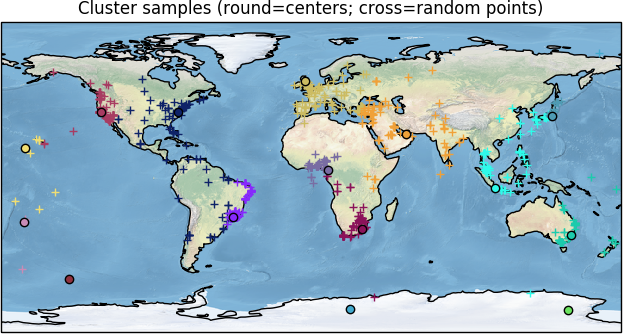
\includegraphics[width=0.9\textwidth]{pictures/map_15_75000_15000_0.png}
		\caption{Map of the initial (static) clustering for the best $\epsilon$ and the best $\beta$}
	\end{subfigure} %
	\begin{subfigure}[t]{0.4\textwidth}
		\centering
		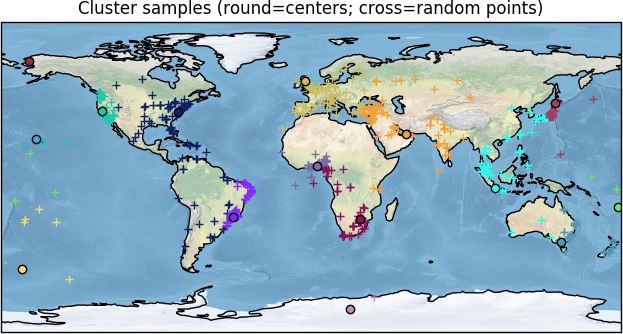
\includegraphics[width=0.9\textwidth]{pictures/map_15_75000_15000_821.png}
		\caption{Map after the first reclustering (here operation $821$) for the best $\epsilon$ and the best $\beta$}
\end{subfigure}
\caption{Spatial representation of the clustering before and after a reclustering operation}
\label{maps}
\end{figure}

\begin{figure}[h]
	\begin{subfigure}[b]{0.3\textwidth}
		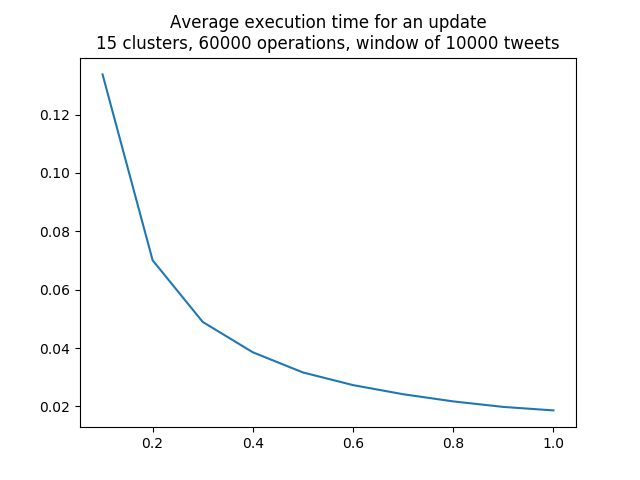
\includegraphics[width=\textwidth]{pictures/average_execution_times_per_update_15_60000_10000.png}
		\caption{Average execution time per update as a function of $\epsilon$}
	\end{subfigure}
	% this comment avoids break-line...
	\begin{subfigure}[b]{0.3\textwidth}
		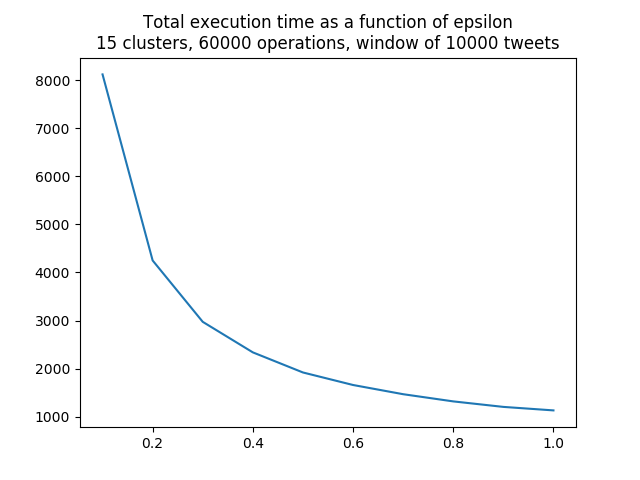
\includegraphics[width=\textwidth]{pictures/final_execution_times_15_60000_10000.png}
		\caption{Total execution time (static and dynamic clustering) as a function of $\epsilon$}
	\end{subfigure}
	%
	\begin{subfigure}[b]{0.3\textwidth}
		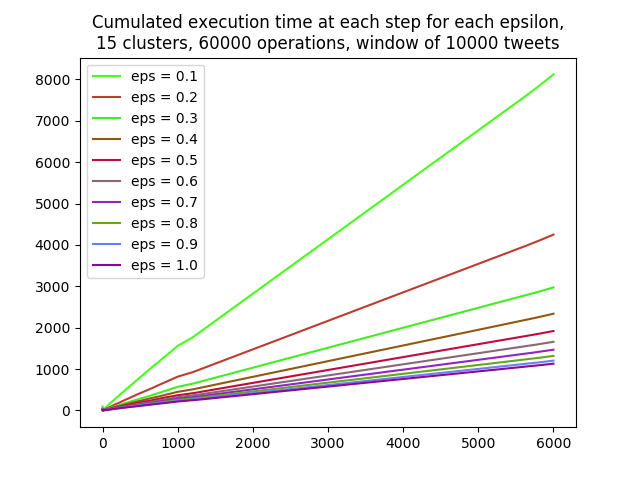
\includegraphics[width=\textwidth]{pictures/cumulated_execution_times_15_60000_10000.png}
		\caption{Evolution of the execution time (sampled each 500 operations)}
	\end{subfigure}
	
	\begin{subfigure}[b]{0.3\textwidth}
		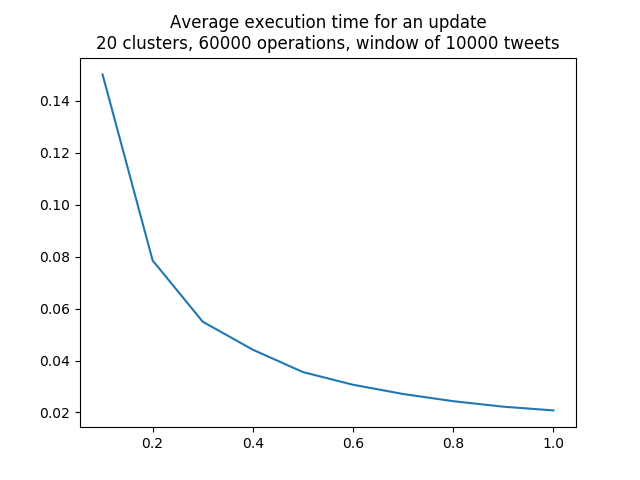
\includegraphics[width=\textwidth]{pictures/average_execution_times_per_update_20_60000_10000.png}
		\caption{Average execution time per update as a function of $\epsilon$}
	\end{subfigure}
	% this comment avoids break-line...
	\begin{subfigure}[b]{0.3\textwidth}
		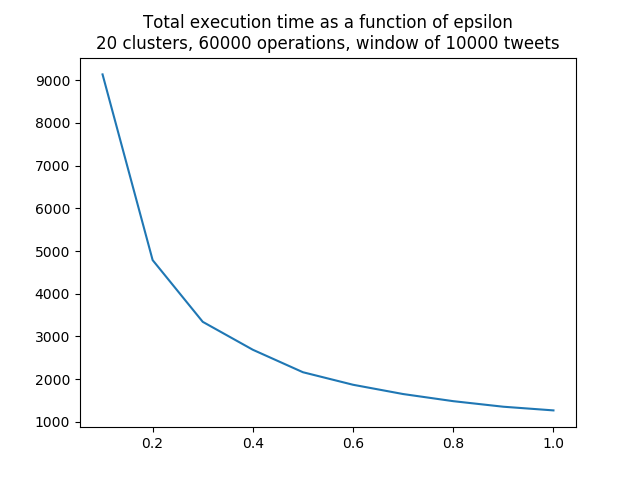
\includegraphics[width=\textwidth]{pictures/final_execution_times_20_60000_10000.png}
		\caption{Total execution time (static and dynamic clustering) as a function of $\epsilon$}
	\end{subfigure}
	%
	\begin{subfigure}[b]{0.3\textwidth}
		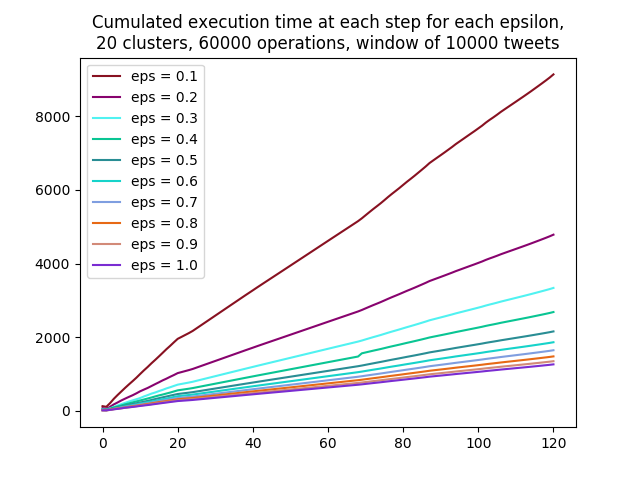
\includegraphics[width=\textwidth]{pictures/cumulated_execution_times_20_60000_10000.png}
		\caption{Evolution of the execution time (sampled each 500 operations)}
	\end{subfigure}
	
	\caption{Experimental results for several sets of parameters ($15$/$20$ clusters, $60000$ operations, $10000$ window width)}\label{fig:ABCD}
\label{plots}
\end{figure}

\begin{figure}
	\centering
	\begin{tabular}{|c|c|c|c|c|c|c|c|c|c|c|c|}
		\hline
		Epsilon & 0.1 & 0.2&0.3&0.4&0.5&0.6&0.7&0.8&0.9&1.0\\ \hline
		Final times & 9139 &	4787 &	3341 &	2687 &	2160 &	1867 &	1649 &	1482 &	1352 &	1266\\
		Ratios &1,91&	1,43&	1,24&	1,24&	1,16&	1,13&	1,11&	1,10&	1,07& \\ \hline	
	\end{tabular}
	\caption{Sensitivities of the execution times to the value of $\epsilon$}
\end{figure}
\begin{figure}
	\centering
	\begin{tabular}{|c|c c c c c c c c c c|}
		\hline
		Offset & 5k & 10k & 15k & 20k & 25k & 30k & 35k & 40k & 45k & 50k\\
		Operations & 45k & 40k & 35k & 30k & 25k & 20k & 15k & 10k & 5k & 0\\ \hline
		F1 scores & 0.47 & 0.59 & 0.60 & 0.57& 0.61 & 0.58 & 0.34 & 0.26 & 0.42 & 1.0 \\ \hline
	\end{tabular}
	\caption{F1 scores for several approximations of window $[50k, 60k[$ with $15$ clusters}
	\label{f1}
\end{figure}
\begin{figure}
	\centering
	\begin{tabular}{|c|c| c |}
		\hline
		Ground truth & Approximation \\ \hline
		2048,40021459 & 2253,24023604 \\ \hline
		Ratio &  0.91 \\ \hline
	\end{tabular}
	\caption{Value of $\beta$ for the window $[30k; 40k]$ with $15$ clusters and $\epsilon = 0.1$ w.r.t its approximation}
	\label{beta_ratio}
\end{figure}
\end{appendices}
\medskip


\bibliography{bibliography}
\bibliographystyle{plain}

\end{document}
